\section{Density Matrix Embedding Theory (DMET)}
我们知道孤立体系BO近似后,其电子$Hamiltonian$量很容易写出
\[\hat{H}_e(\mathbf{R})=-\frac{1}{2}\sum_{i=1}^{N_e}\nabla_i^2-\sum_{I=1}^{N_N}\sum_{i=1}^{N_e}\frac{Z_I}{|\mathbf{R}_I-\mathbf{r}_i|}+\sum_{i>j}^{N_e}\frac{1}{|\mathbf{r}_i-\mathbf{r}_j|}+\sum_{I>J}^{N_N}\frac{Z_IZ_J}{|\mathbf{R}_I-\mathbf{R}_J|} \tag{1}\]
假设我们拿到了满足包含上述$Hamiltonian$量的薛定谔方程的波函数$\ket*{\Psi_e}$:
\[\hat{H}_e(\mathbf{R})\left|\Psi_e(\mathbf{r};\mathbf{R})\right\rangle=E_{e;n}(\mathbf{R})\left|\Psi_e(\mathbf{r};\mathbf{R})\right\rangle \]
在二次量子化的语言下,$\ket*{\Psi_e}$可以被写成:
\[\ket*{\Psi_e}=a_1^{\dagger}a_2^{\dagger}\cdots a_n^{\dagger}\ket{}\]
整个系统中我们感兴趣的部分可能只与一小部分电子有关(就算是关系能量之类的整体性质也能拆成小块遍历(也许可能大概),记为fragment $\ket{\alpha_p}=\alpha_p^{\dagger}\ket{} \ (p=1,2,\cdots,m)$,其余部分记为environment $\ket{\beta_p}=\beta_p^{\dagger}\ket{} \ (p=m+1,m+2,\cdots,n)$。
那么自然而然,系统在粒子数表象下的总Fock空间可以被fragment和environment的两个子空间张量积表示:
\[V_{f+e} = V_f \otimes V_e\]
则全空间的中的一个多电子波函数(在mean field语境下是一个行列式)可以被如下表示:
\[\ket{\Psi}=\sum_{i=1}^{m}\sum_{j=m+1}^{n}c_{ij}\ket{\alpha_i}\otimes\ket{\beta_j}\]
我们可以发现该波函数在这个基底下的系数矩阵$\mathbf{C}=[c_{ij}]_{m \times (n-m)}$,可以做SVD分解:
\[\mathbf{C}=\mathbf{U}\mathbf{\Lambda}\mathbf{V}^{\dagger} \quad , \quad c_{ij}=\sum_{p=1}^{\min\{m,n-m\}}U_{ip}\Lambda_{pp}V_{jp}^*\]
我们一般希望$m<<n$ (废话,于是我们可以进一步进行变换
\[\ket{\Psi}=\sum_{i=1}^{m}\sum_{j=m+1}^{n}\sum_{p=1}^mU_{ip}\Lambda_{pp}V_{jp}^*\ket{\alpha_i}\otimes\ket{\beta_j}=\sum_{p=1}^{m}\Lambda_{pp}\left(\sum_{i=1}^{m}U_{ip}\left|\alpha_i\right>\right)\otimes\left(\sum_{j=1}^{n-m}V_{jp}^*\left|\beta_j\right>\right)=\sum_{p=1}^m\Lambda_{pp}\ket{f_p}\otimes\ket{b_p}\]
上述变换没有任何近似,这意味着除了fragment只与environment中数量相同的粒子有直接纠缠,\href{https://dspace.mit.edu/handle/1721.1/147265}{我们可以以一种更紧凑的方式表达波函数}。
则密度矩阵可以表示为:
\[\hat{D}=\ket*{\Psi}\bra*{\Psi} = \sum_{p=1}^m \sum_{q=1}^m \Lambda_{pp}\ket{f_p}\otimes\ket{b_p}\Lambda_{qq}\bra{f_q}\otimes\bra{b_q}\]

出于算得动的考虑,我们将mean-field波函数作初始波函数,比如HF波函数。

因为实际计算中,HF一般会使用1-RDM进行运算,所以我们在1-RDM中进行操作。
出于方便考虑,我们可以选取变换使得$\{\ket{f_p}\otimes\ket{b_p}\}$正交归一,叫做embedding basis (EO),则1-RDM算符在该表象下为:
\[\hat{D}=\sum_i^{\text{occ}}n_i\ket*{\psi_i}\bra*{\psi_i} = \sum_{p=1}^m \Lambda_{p}^2\ket{f_p}\otimes\ket{b_p}\bra{f_p}\otimes\bra{b_p}\]

更进一步,如果我们一开始就使用localization或者orthonormal orbitals作为1-RDM的基底,那么可以直接取$\ket{f_p}=\ket{\alpha_p}$,即$\mathbf{U}=\mathbf{I}$,直接计算矩阵元,这里用了$\Lambda_p^2=0,1$是$\ket{f_p},\ket{b_p}$在偏迹算符下的共同本征值:
\[\hat{\rho}_f=\sum_k\bra{b_k}\ket{\Psi}\bra{\Psi}\ket{b_k}=\sum_k\ket{f_k}\Lambda_{b,k}^2\bra{f_k}\]
\[\hat{\rho}_b=\sum_k\bra{f_k}\ket{\Psi}\bra{\Psi}\ket{f_k}=\sum_k\ket{b_k}\Lambda_{f,k}^2\bra{b_k}\]
因为施密特分解要求$\{\ket{f_k}\},\{\ket{b_k}\}$正交归一,所以可以放心插入下标:
\[\bra{\alpha_i}\hat{D}\ket{\alpha_j} = \sum_{kl}\bra{\alpha_i}\ket{f_k}\bra{f_k}\hat{D}\ket{f_l}\bra{f_l}\ket{\alpha_j} =\Lambda_{f,i}^2\delta_{ij}\]
\[\bra{\beta_i}\hat{D}\ket{\beta_j} = \sum_{kl}\bra{\beta_i}\ket{b_k}\bra{b_k}\hat{D}\ket{b_l}\bra{b_l}\ket{\beta_j} =\Lambda_{b,i}^2\delta_{ij}\]
\[\bra{\alpha_i}\hat{D}\ket{\beta_j} = \sum_{kl}\bra{\alpha_i}\ket{f_k}\bra{f_k}\hat{D}\ket{b_l}\bra{b_l}\ket{\beta_j} =\Lambda_{f,i}\Lambda_{b,j}V_{ij}\]
\[\bra{\beta_i}\hat{D}\ket{\alpha_j} = \sum_{kl}\bra{\beta_i}\ket{b_k}\bra{b_k}\hat{D}\ket{f_l}\bra{f_l}\ket{\alpha_j} =\Lambda_{b,i}\Lambda_{f,j}V^{\dagger}_{ij}\]

从LO $\{\ket{\alpha_p}\otimes\ket{\beta_p}\}$ 变换到 EO $\{\ket{f_p}\otimes\ket{b_p}\}$如下图所示。
\begin{figure}[htbp]
    \centering
    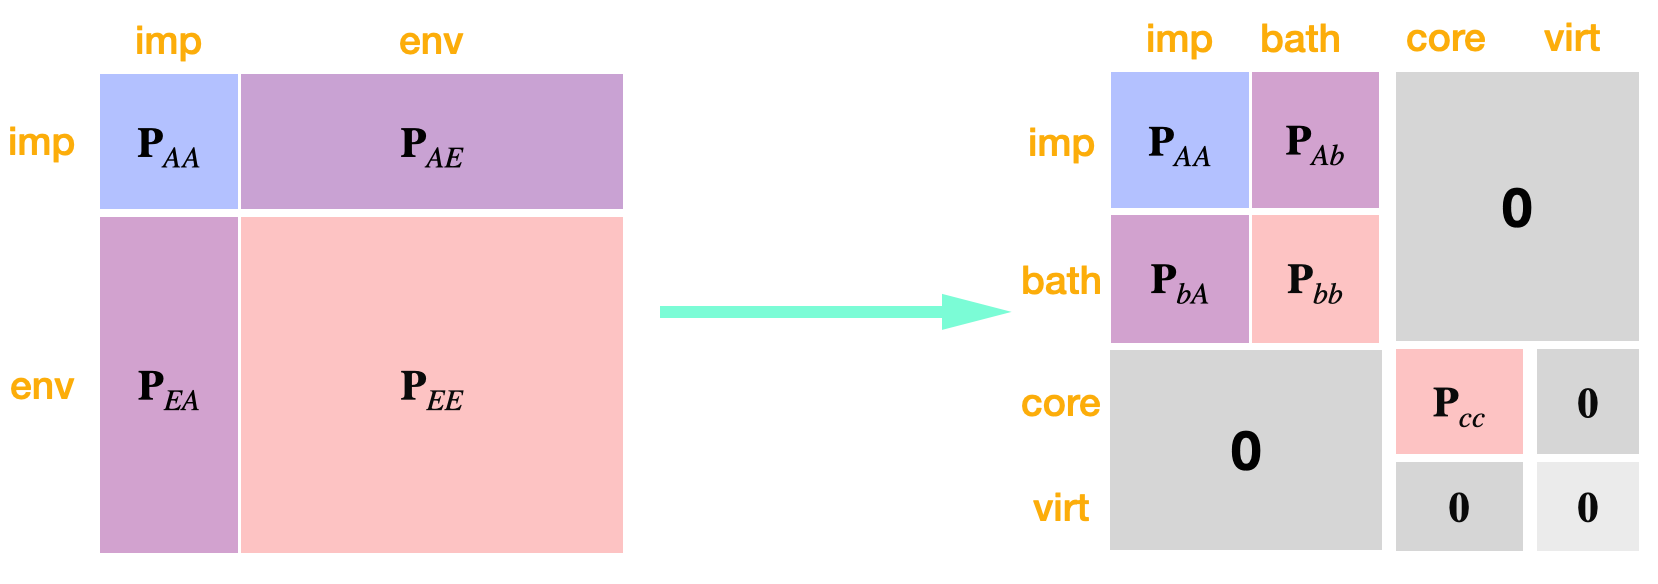
\includegraphics[scale=0.5]{./fig/et/dmet-hartree-fock-dm.png}
    \caption{DMET对从LO到EO的变换示意图}
\end{figure}

如果直接对1-RDM中$\mathbf{P}_{AE}$部分的SVD分解,则有(SVD分解不唯一,所以从1-RDM做分解和从系数矩阵做分解是等价的操作)
\[\mathbf{P}_{AE}=\mathbf{U}_{new}\mathbf{\Lambda}_{new}\mathbf{V}_{new}^{\dagger}=\mathbf{\Lambda}_f\mathbf{\Lambda}_b \mathbf{V}\]

至此我们统一了两种常见的DMET表述方式。